\chapter{Implementation}
 
\section{PTU TASS library}
\subsection{Stabilise command}
\label{stabilize_implementation}
 This is a relatively simple task since it just requires for the two digits to be added to the final message and sent to the PTU. However before doing this project I didn't know much about the ASCII table. I ended up spending a significant amount of time reading and rereading PTU documentation
 
 ~\ref{fig:pushDfunction}
 
 \begin{figure}[H]
 \centering
 \centerline{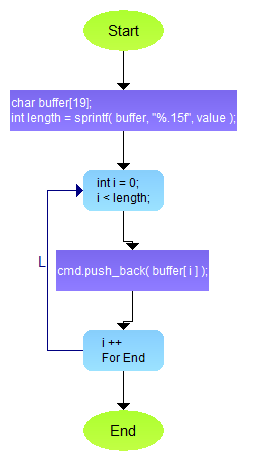
\includegraphics[scale=0.65]{./images/pushDfunction}}
 \caption{Flow for the function to translate doubles in to the ASCII encoding}
 \label{fig:pushDfunction}
 \end{figure}
 \subsubsection{drift rate calculation}
 
 The algorithm presented below will work only if we assume that vertical position of the PTU platform is desired. It does not accommodate the case when the PTU  platform is stabilized at the position other that vertical. This was found at the time of writing report and could be fixed given the more time.